\documentclass[12pt,a4paper,table]{article}

\usepackage[a4paper,
            tmargin=2cm,
            bmargin=2cm,
            lmargin=2cm,
            rmargin=2cm,
            bindingoffset=0cm]{geometry}

\usepackage{lmodern}
\usepackage[T1]{polski}
\usepackage[utf8]{inputenc}
\usepackage{tocloft}
\usepackage{hyperref}
\usepackage{amsmath}
\usepackage{listings}
\usepackage{graphicx}
\usepackage{subfig}
\usepackage{float}
\usepackage{booktabs}

\hypersetup{
    colorlinks,
    citecolor=black,
    filecolor=black,
    linkcolor=black,
    urlcolor=black
}

\newtheorem{definition}{Def}


\begin{document}
    \title {
        Teoria współbieżności
        Sieci Petriego
    }

    \author{
        Przemysław Węglik
    }

    \date{\today}

    \maketitle

    \section{Zadanie 1}
    Sieć może wyprodukować nieskończoność znaczników w miejscu P2, ale
    liczba znacznikþw które pojawią się w P4, jest ograniczona początkowym znaczeniem P3.
    \begin{figure}[H]
        \centering
        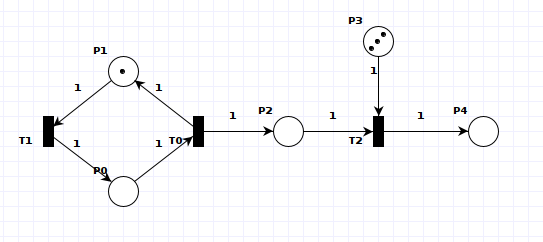
\includegraphics[width=0.6\linewidth]{img/zad1-1.png}
        \caption{Sieć Petriego}
        \label{fig:zad1-1}
    \end{figure}

    \begin{figure}[H]
        \centering
        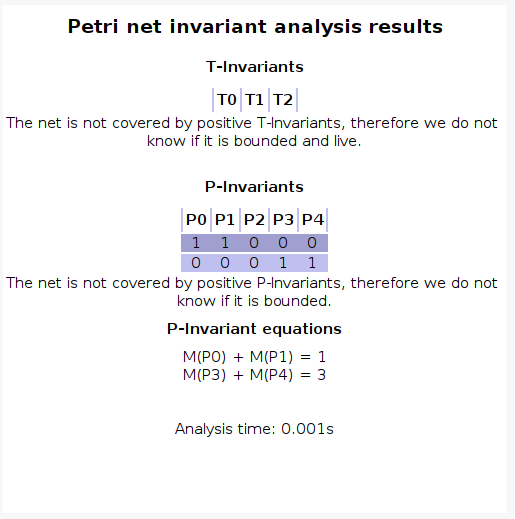
\includegraphics[width=0.6\linewidth]{img/zad1-2.png}
        \caption{Analiza niezmienników}
        \label{fig:zad1-2}
    \end{figure}

    Sieć nie jest pokryta pozytywnymi niezmiennikami miejsc, a zatem nie wiadomo
    czy jest ogarniczona. Obserwując sieć widzimy, że nie jest (w P2 może się znaleźć
    nieskończenie wiele znaczników).

    Jeśli chodzi o niezmienniki miejsc to ponownie potwierdzają się początkowe informacje.
    Jeden ze zbiorów niezmienników zawiera P0 i P1, ponieważ tworzą cykl który nie 
    zmienia w nich liczby znaczników.
    Drugim zbiorem jest P3 i P4, ponieważ każde zmniejszenie liczby znaczników w P3 skutukuje
    przybyciem zniacznika do P4.


    \begin{figure}[H]
        \centering
        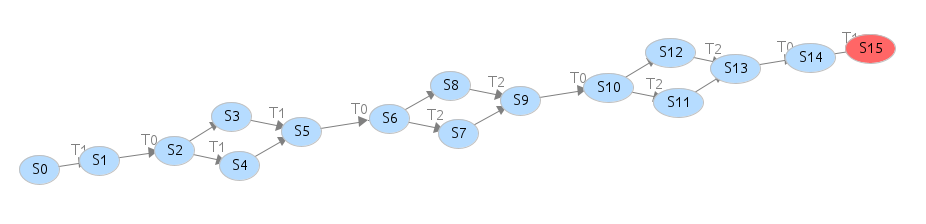
\includegraphics[width=1\linewidth]{img/zad1-3.png}
        \caption{Graf osiągalności}
        \label{fig:zad1-3}
    \end{figure}

    Dla potrzeb ogarniczenia rozamiru grafu nałożyłem ogarniczenie pojemności = 1 na P2.
    Tranzycje następują w oczekiwanej kolejności. Po wyczerpaniu znaczników z P3, sieć
    znajduje się w takim stanie, że może w nieskończoność odpalać tranzycje T0 i T1, oc symbolizuje czerwony kolor na rysunku


    \section{Zadanie 2}

    Sieć reprezentuje swego rodzaju zliczanie ile razy został wykonany cykl operacji.

    \begin{figure}[H]
        \centering
        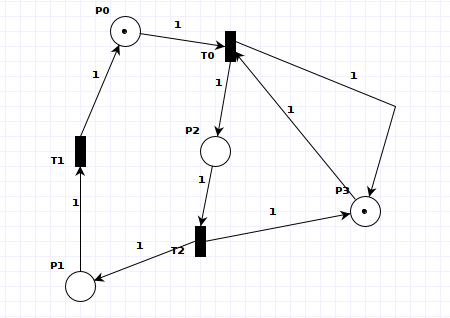
\includegraphics[width=0.6\linewidth]{img/zad2-1.png}
        \caption{Sieć Petriego}
        \label{fig:zad2-1}
    \end{figure}

    \begin{figure}[H]
        \centering
        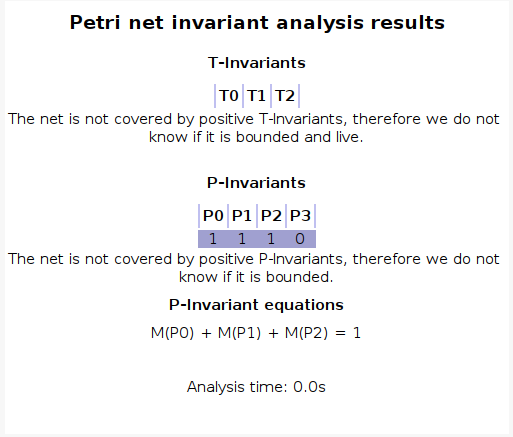
\includegraphics[width=0.6\linewidth]{img/zad2-2.png}
        \caption{Analiza niezmienników}
        \label{fig:zad2-2}
    \end{figure}

    \textbf{Sieć nie jest odwracalna}, bo wtedy niezmienniki tranzycji pokazałyby jakie tranzycje trzeba wykonać
    w tym celu. Sieć nie jest pokryta takimi niezmiennikami.

    \begin{figure}[H]
        \centering
        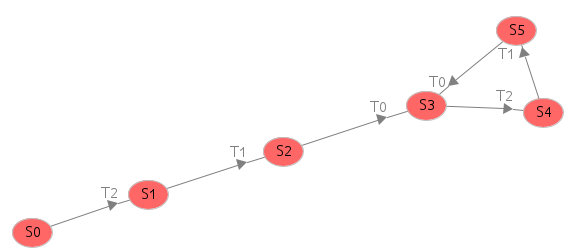
\includegraphics[width=0.6\linewidth]{img/zad2-3.png}
        \caption{Graf osiągalności}
        \label{fig:zad2-3}
    \end{figure}

    \textbf{Sieć nie jest ogarniczona}, liczba znaczników możne rosnąć do nieskończoności w cyklu między stanami
    S3, S4 i S5.

    \textbf{Sieć jest żywa}, ponieważ zawsze możemy odpalić którąś z tranzycji.

    \section{Zadanie 3}

    \begin{figure}[H]
        \centering
        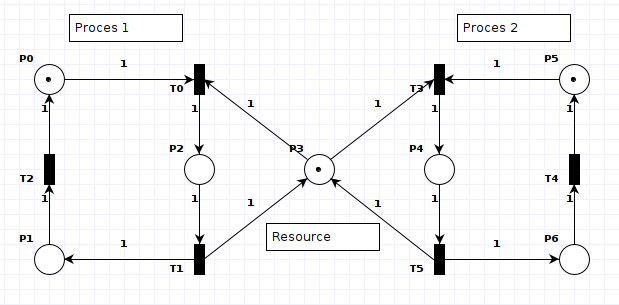
\includegraphics[width=0.8\linewidth]{img/zad3-1.png}
        \caption{Sieć Petriego}
        \label{fig:zad3-1}
    \end{figure}

    \begin{figure}[H]
        \centering
        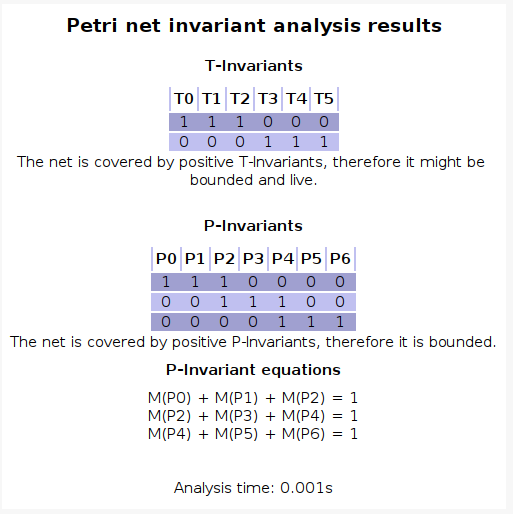
\includegraphics[width=0.6\linewidth]{img/zad3-2.png}
        \caption{Analiza niezmienników}
        \label{fig:zad3-2}
    \end{figure}

    Widzimy czy zbiory w analizie P-niezmienników. Zbiory pierwszy i trzeci odpowiadają ciągłości
    obliczeń w procesach. Zbiór drugi reprezentuje ochronę zasobu. 
    Ilość znaczników między miejscami P2, P3 i P4 się nie zmienia. Jeśli obecność znacznika oznacza
    kontrolę nad zasobem to w elegancki sposób medluje to przyznawanie dostępu do zasobu.

    \section{Zadanie 4}

    \begin{figure}[H]
        \centering
        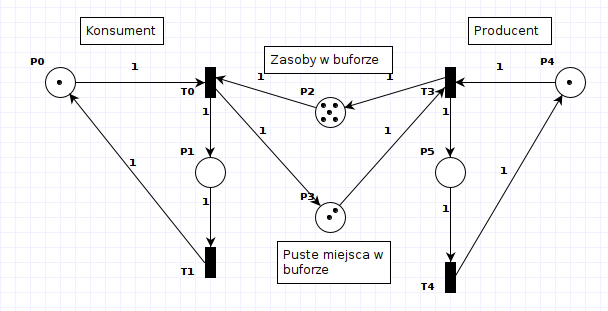
\includegraphics[width=0.8\linewidth]{img/zad4-1.png}
        \caption{Sieć Petriego}
        \label{fig:zad4-1}
    \end{figure}

    \begin{figure}[H]
        \centering
        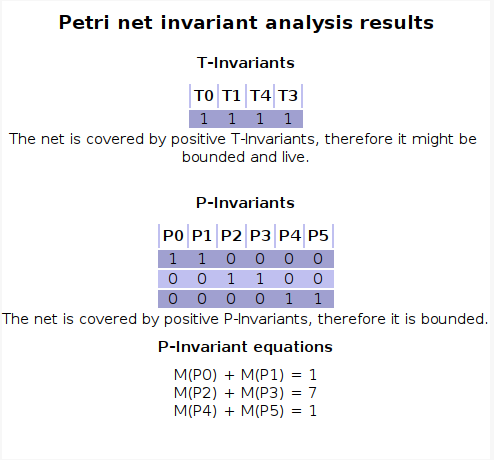
\includegraphics[width=0.6\linewidth]{img/zad4-2.png}
        \caption{Analiza niezmienników}
        \label{fig:zad4-2}
    \end{figure}

    \textbf{Sieć jest zachowawcza}, ponieważ jest pokryta pozytywnymi niezmiennikami 
    pozycji. W każdym ze zbiorów liczba znaczników się nie zmienia, a że przykrywają sobą całą sieć,
    to możemy wniskować, że suma znaczników w całej sieci również się nie zmienia.

    Mówi nam o tym równanie drugie. Rozmiar bufora w przykładzie to 7.

    \section{Zadanie 5}

    \begin{figure}[H]
        \centering
        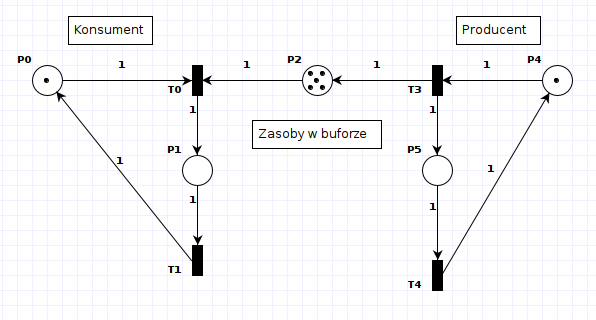
\includegraphics[width=0.8\linewidth]{img/zad5-1.png}
        \caption{Sieć Petriego}
        \label{fig:zad5-1}
    \end{figure}

    \begin{figure}[H]
        \centering
        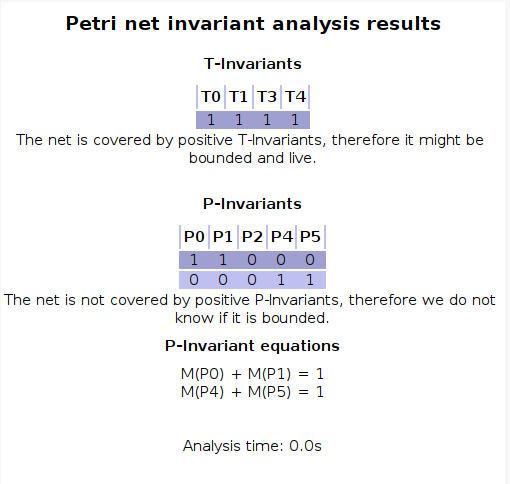
\includegraphics[width=0.6\linewidth]{img/zad5-2.png}
        \caption{Analiza niezmienników}
        \label{fig:zad5-2}
    \end{figure}

    \textbf{Sieć nie jest zachowawcza}, ponieważ w P2 liczba znaczników nie jest ograniczona.
    Co ciekawe, z analizy niezmienników miejsc wynika, że \textbf{sieć jest odwracalna}.

    \section{Zadanie 6}

    \begin{figure}[H]
        \centering
        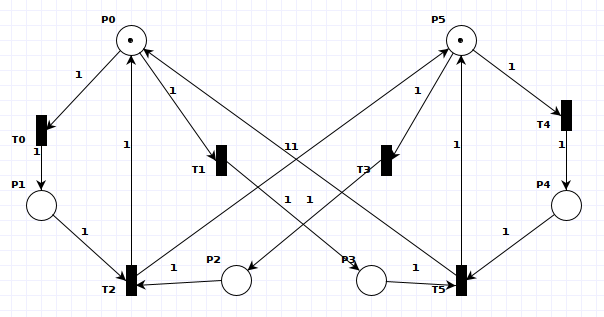
\includegraphics[width=0.8\linewidth]{img/zad6-1.png}
        \caption{Sieć Petriego}
        \label{fig:zad6-1}
    \end{figure}

    \begin{figure}[H]
        \centering
        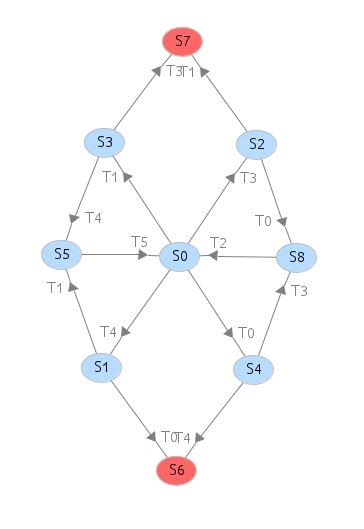
\includegraphics[width=0.6\linewidth]{img/zad6-2.png}
        \caption{Graf osiągalności}
        \label{fig:zad6-2}
    \end{figure}

    Występuje zakleszczenie w stanach S6 i S7. Odpowiadają one znaczeniom:
        S6 - \{0, 1, 0, 0, 1, 0\}, S7 - \{0, 0, 1, 1, 0, 0\}. Oznacza to zakleszczenie Występuje
        gdy znaczniki znajdą się jednoczenie w miejscach P1 i P4 lub P2 i P3.

    \begin{figure}[H]
        \centering
        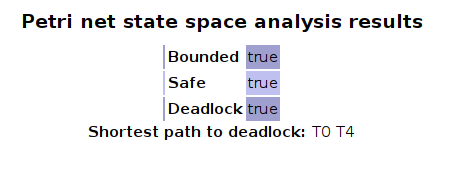
\includegraphics[width=0.6\linewidth]{img/zad6-3.png}
        \caption{State Space Analysis}
        \label{fig:zad6-3}
    \end{figure}

    State Space Analysis potwierdza naszą analizę i wskazuje najkrótszą scieżkę do
    zakleszczenia jako wykonanie tranzycji T0 i T4, co prowadzi nas do stanu S6

    \section{Zadanie 7}

    \begin{figure}[H]
        \centering
        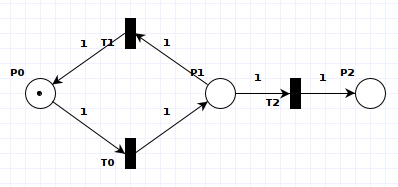
\includegraphics[width=0.8\linewidth]{img/zad7-1.png}
        \caption{Sieć Petriego}
        \label{fig:zad7-1}
    \end{figure}

    \begin{figure}[H]
        \centering
        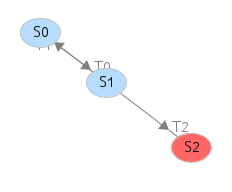
\includegraphics[width=0.6\linewidth]{img/zad7-2.png}
        \caption{Graf osiągalności}
        \label{fig:zad7-2}
    \end{figure}

    \begin{figure}[H]
        \centering
        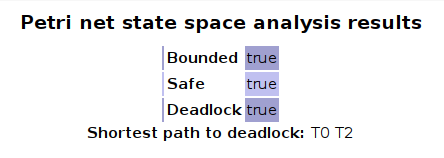
\includegraphics[width=0.6\linewidth]{img/zad7-3.png}
        \caption{State Space Analysis}
        \label{fig:zad7-3}
    \end{figure}

    Analiza jest bardzo prosta. Sieć zakleszcza się w stanie S2, które odpowiada znaczeniu, w którym
    znacznik znajduje się w P2. Nie może stamtąd przejść za pomocą żadnej tranzycji i następuje zakleszczenie.

    State Space Analysis potwierdza naszą analizę.


    \section{Zadanie 8}

    \begin{figure}[H]
        \centering
        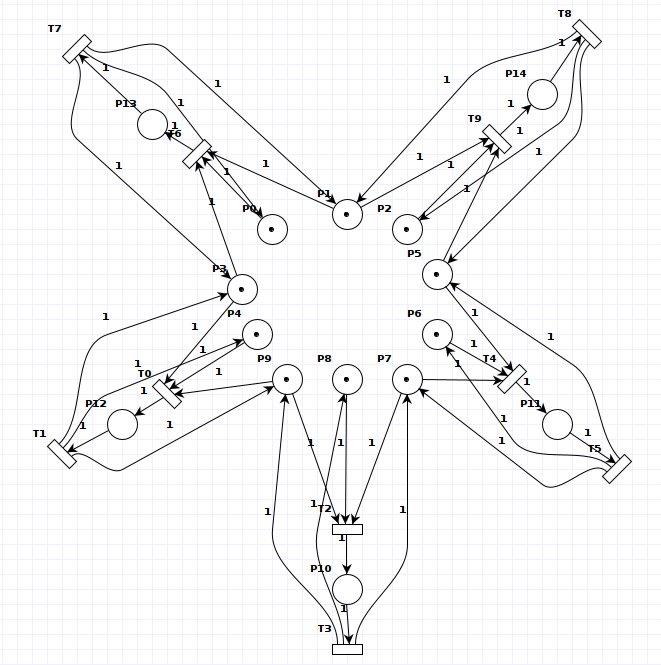
\includegraphics[width=1\linewidth]{img/zad8-1.png}
        \caption{Sieć Petriego}
        \label{fig:zad8-1}
    \end{figure}

    \begin{figure}[H]
        \centering
        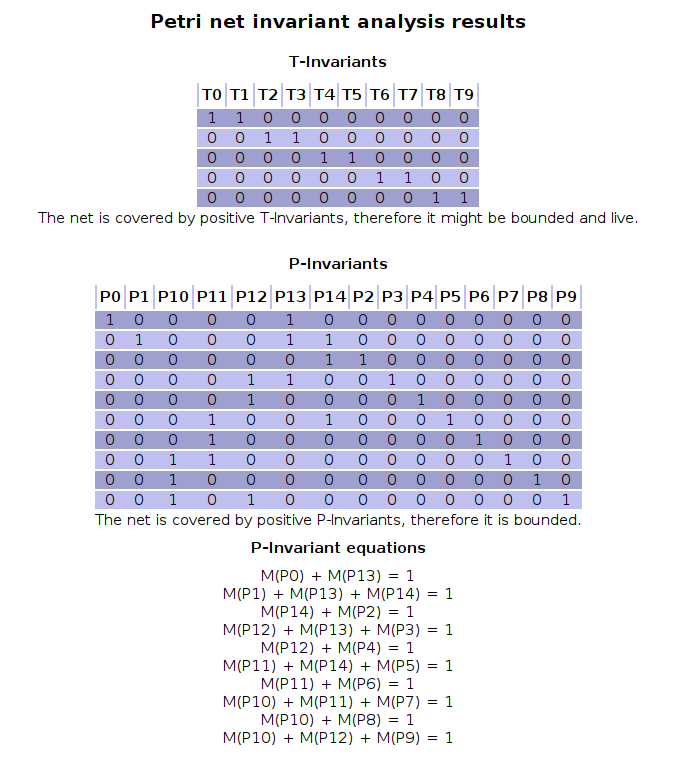
\includegraphics[width=0.8\linewidth]{img/zad8-2.png}
        \caption{Analiza niezmienników}
        \label{fig:zad8-2}
    \end{figure}

    \begin{figure}[H]
        \centering
        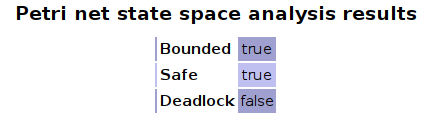
\includegraphics[width=0.6\linewidth]{img/zad8-3.png}
        \caption{State Space Analysis}
        \label{fig:zad8-3}
    \end{figure}

    Wnioskujemy, że \textbf{sieć jest ograniczona, zachowawcza i bezpieczna.}
    Nie występują zakleszczenia.

    Analizując logicznie co się dzieje w sieci widzimy, że zbudowana jest ona z modułów reprezentujących
    filozofów i z miejsc reprezentujących widelce. Znacznik w takim miejscu oznacza, że widelec lezy na stole,
    a jego brak, że któryś z filozofów obecnie go używa.

    Przeanalizujmy filozofa który "składa się" z P4, P12, T0 i T1.
    Znacznik w P4 odpowiada sytuacji gdy filozof czeka na oba widelce. Odpalając T0 filozof podnosi widelce
    i ustawia znacznik w P12, co oznacza, że aktualnie używa widelców. Odpalając T1 filozof odkłada oba widelce na miejsce.



\end{document}